\documentclass{beamer}

\mode<presentation>
{
	\usetheme{Warsaw}
	\usepackage{graphicx}
	% or ...	
	
	\setbeamercovered{transparent,invisible}
	\setbeamertemplate{navigation symbols}{}
	% or whatever (possibly just delete it)
}

\usepackage[english]{babel}
% or whatever
\usepackage{graphicx,subfigure}
\usepackage[utf8]{inputenc}
% or whatever

\usepackage{times}
\usepackage[T1]{fontenc}
% Or whatever. Note that the encoding and the font should match. If T1
% does not look nice, try deleting the line with the fontenc.
\usepackage{amsthm}
\newtheorem*{mylim*}{Limitations}
\usepackage{gensymb}
\usepackage{hyperref}
\hypersetup{
	colorlinks=true,
	linkcolor=blue,
	anchorcolor=blue,
	filecolor=blue,      
	citecolor=blue,
	urlcolor=blue
}
\usepackage{url,graphicx,subfigure}
\usepackage{listings}
\usepackage{color}
\usepackage{soul}
\usepackage{xspace}
\usepackage{pifont}
\usepackage{cite}
\usepackage{lipsum}% http://ctan.org/pkg/lipsum
\usepackage{algpseudocode}% http://ctan.org/pkg/algorithmicx
\usepackage{graphicx}
\usepackage[compatibility=false]{caption}% http://ctan.org/pkg/caption
\usepackage{booktabs}
\usepackage{url}
\usepackage{multirow}
\usepackage{pgfplots}
\usepackage{tikz}
\usetikzlibrary{matrix,fit,shapes,calc,positioning,shadows,arrows,shapes,backgrounds,decorations.markings,fadings}
\usepgfplotslibrary{statistics}
\usepackage[normalem]{ulem}
\useunder{\uline}{\ul}{}
\usepackage[skins]{tcolorbox}
\usepackage[linesnumbered,lined,boxed,ruled,vlined]{algorithm2e}
\usepackage[labelformat=empty]{caption}
\usepackage{color, colortbl}
\definecolor{Gray}{gray}{0.9}
\usepackage{amsmath,amssymb,amsfonts}

\hyphenation{op-tical net-works semi-conduc-tor}

\definecolor{comments}{rgb}{0.25,0.5,0.35}

\definecolor{brass}{rgb}{0.71, 0.65, 0.26}

\definecolor{SM}{rgb}{0.5,0,1}
\newcommand {\rsm} {\color{SM}}

\newcommand{\disp}{\insertframenumber/\inserttotalframenumber}

\newcommand{\backupbegin}{
	\newcounter{finalframe}
	\setcounter{finalframe}{\value{framenumber}}
}
\newcommand{\backupend}{
	\setcounter{framenumber}{\value{finalframe}}
}

\definecolor{antiquefuchsia}{rgb}{0.7, 0.1, 0.85}
\definecolor{airforceblue}{rgb}{0.36, 0.54, 0.66}
\definecolor{brass}{rgb}{0.71, 0.65, 0.26}
\definecolor{indiagreen}{rgb}{0.07, 0.53, 0.03}
\definecolor{darkorange}{rgb}{1.0, 0.55, 0.0}
\definecolor{navyblue}{rgb}{0.36, 0.54, 0.66}
\definecolor{darkred}{rgb}{0.55, 0.0, 0.0}

\newcommand{\REM}[1]{}
\newcommand{\todo}[1]{\textrm{\color{blue} #1}}
\newcommand{\sm}[1]{\textrm{\color{red} #1}}
\newcommand{\colosseum}{\textsf{Colosseum}\xspace}
\newcommand{\hansie}{\textsf{Hansie}\xspace}
\newcommand{\mahtab}{\textsf{Mahtab}\xspace}
\newcommand{\overallspeedup}{\todo{XXX}}

\resetcounteronoverlays{algocf}

\newcommand{\smr}[1]{\textrm{\color{black} #1}}
\newcommand{\sms}[1]{\textrm{\color{black} #1}}
\renewcommand{\ttdefault}{pcr}
\lstset{
	language=Java,
	escapechar=|,
	numbers=left,
	stepnumber=1,
	numbersep=5pt,
	numberstyle=\tiny\color{gray},
	backgroundcolor=\color{white},
	stringstyle=\fontsize{7.5}{7.5}\selectfont\ttfamily,
	keywordstyle=\ttfamily,
	showspaces=false,
	showstringspaces=false,
	showtabs=false,
	tabsize=2,
	captionpos=b,
	breaklines=true,
	breakatwhitespace=true,
	title=\lstname,
	basicstyle=\fontsize{7.5}{7.5}\selectfont\ttfamily,
	commentstyle=\color{red},
}
\newcommand{\ie}{i.e.}
\newcommand{\eg}{e.g.}
\newcommand{\aka}{a.k.a.}
\newcommand{\etal}{et al.}  % and colleagues
\newcommand{\CodeIn}[1]{{\small{\texttt{#1}}}}
\newcommand{\CodeInTab}[1]{{\scriptsize{\texttt{#1}}}}
\newcommand{\FancyIn}[1]{{\small{\textsc{#1}}}}
\newcommand{\MyComment}[1]{}
% common names
\newcommand{\reveng}{Reverse Engineering}

%% review original
\newcommand{\Fix}[1]{{\textbf{[[}\color{magenta}#1}\textbf{]]}}
\newcommand{\Mar}[1]{{\textbf{[[Marcelo:~}\color{red}#1}\textbf{]]}}
\newcommand{\SM}[1]{{\textbf{[[Shouvick:~}\color{blue}#1}\textbf{]]}}
\newcommand{\Den}[1]{[\textbf{Denini}:~{\color{brown} #1}]}

% \newcommand{\Fix}[1]{}
% \newcommand{\Mar}[1]{}
% \newcommand{\SM}[1]{}
% \newcommand{\Den}[1]{}

%% numbers
\newcommand{\configClasses}{\CodeIn{classes}}
\newcommand{\configMethods}{\CodeIn{methods}}
\newcommand{\configClassesAndMethods}{\CodeIn{classesMethods}}
\newcommand{\configClassesTab}{\CodeInTab{classes}}
\newcommand{\configMethodsTab}{\CodeInTab{methods}}
\newcommand{\configClassesAndMethodsTab}{\CodeInTab{classesMethods}}

\newcommand{\tname}{\textsc{PASTE}}

\def\denseitems{
   \itemsep1pt plus1pt minus1pt
   \parsep0pt plus0pt
   \parskip0pt\topsep0pt}

%% numbers and names
\newcommand{\OurURL}{\url{https://github.com/STAR-RG/paste}}
\newcommand{\NumProjects}{25}
\newcommand{\NumProjectsSpeedups}{13}
\newcommand{\FrequencySpeedups}{52} % NumProjectsSpeedups/NumProjects (13/25)
\newcommand{\SpeedupClassesAvg}{1.47}
\newcommand{\SpeedupClassesMedian}{1.59}
\newcommand{\SpeedupClassesMax}{2.28}
\newcommand{\SpeedupClassesMin}{0.93}
\newcommand{\NumRepeatsExperiment}{5}
\newcommand{\NumRepeatsManifest}{10}
\newcommand{\NumProjectsParExecFails}{11}
\newcommand{\NumProjectsParExecFailsPercentage}{44}
\newcommand{\NumStars}{200}
\newcommand{\NumTests}{300}
\newcommand{\NumFailsAtlasStageOneMethods}{147.2}
\newcommand{\NumFailsAtlasStageOneMethodsNoFraction}{141.2}
\newcommand{\NumFailsAtlasStageTwoMethods}{6}
\newcommand{\NumFailsClassesTotalStageOne}{402.6}
\newcommand{\NumFailsClassesAndMethodsTotalStageOne}{731.2}
\newcommand{\NumFailsMethodsTotalStageOne}{879.6}
\newcommand{\NumTestsClassificationSearchProcessorTest}{10}
\newcommand{\NumTestsMillionsPerDayGoogle}{150}
\newcommand{\EpochDuration}{45}
\newcommand{\NumDigitsSHA}{7}
\newcommand{\Processor}{Intel Core i5-1035G1 CPU @ 1.00GHz (base frequency)}
\newcommand{\NumCPUs}{8}
\newcommand{\NumCores}{4}
\newcommand{\RAMCapacity}{8}
\newcommand{\HardDiskCapacity}{512}
\newcommand{\KernelVersion}{5.4.0-42-generic}
\newcommand{\JavaVersion}{1.8.0\_282}
\newcommand{\BashVersion}{5.0.17}
\newcommand{\MavenVersion}{3.6.3}
\newcommand{\NumDepsChronicleQueue}{251}
\newcommand{\NumTestsChronicleQueue}{338}
\newcommand{\NumDepsCommonsCcollection}{2}
\newcommand{\NumTestsCommonsCcollection}{16,923}
\newcommand{\ForkscriptSurefirePatchedVersion}{\CodeIn{maven-surefire-plugin v3.0.0-M5}}
%% names


%% Configuration modes from ASE
\newcommand{\Seq}{\CodeIn{sequential}}
\newcommand{\SeqClassParMeth}{\configClasses}
\newcommand{\ParClassSeqMeth}{\configMethods}
\newcommand{\ParClassParMeth}{\configClassesAndMethods}
\newcommand{\Fork}{\Fix{?}}
\newcommand{\ForkSeq}{\Fix{?}}
\newcommand{\ForkParMeth}{\Fix{?}}
\newcommand{\pomf}{\CodeIn{pom.xml}}



\title[\color{white}ICSME 2021 Research Track Presentation.\hspace{14mm}\disp] % (optional, use only with long paper titles)
{Soundy Automated Parallelization\\of Test Execution}

\author[Shouvick Mondal \textit{et al}.] % (optional, use only with lots of authors)
{\underline{Shouvick Mondal}, Denini Silva, Marcelo d'Amorim\\\vspace{2mm}
{\scriptsize IIT Madras (India), UFPE (Brazil), UFPE (Brazil)}
\\\vspace{2mm}
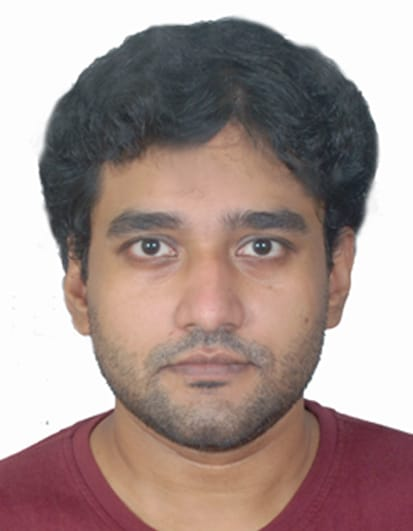
\includegraphics[width=0.13\textwidth]{images/shouvick2.jpg}~~~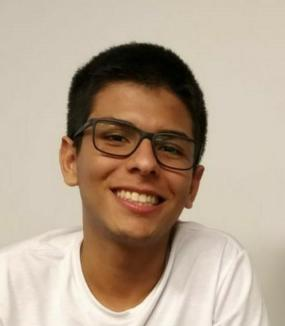
\includegraphics[width=0.15\textwidth]{images/denini.jpg}~~~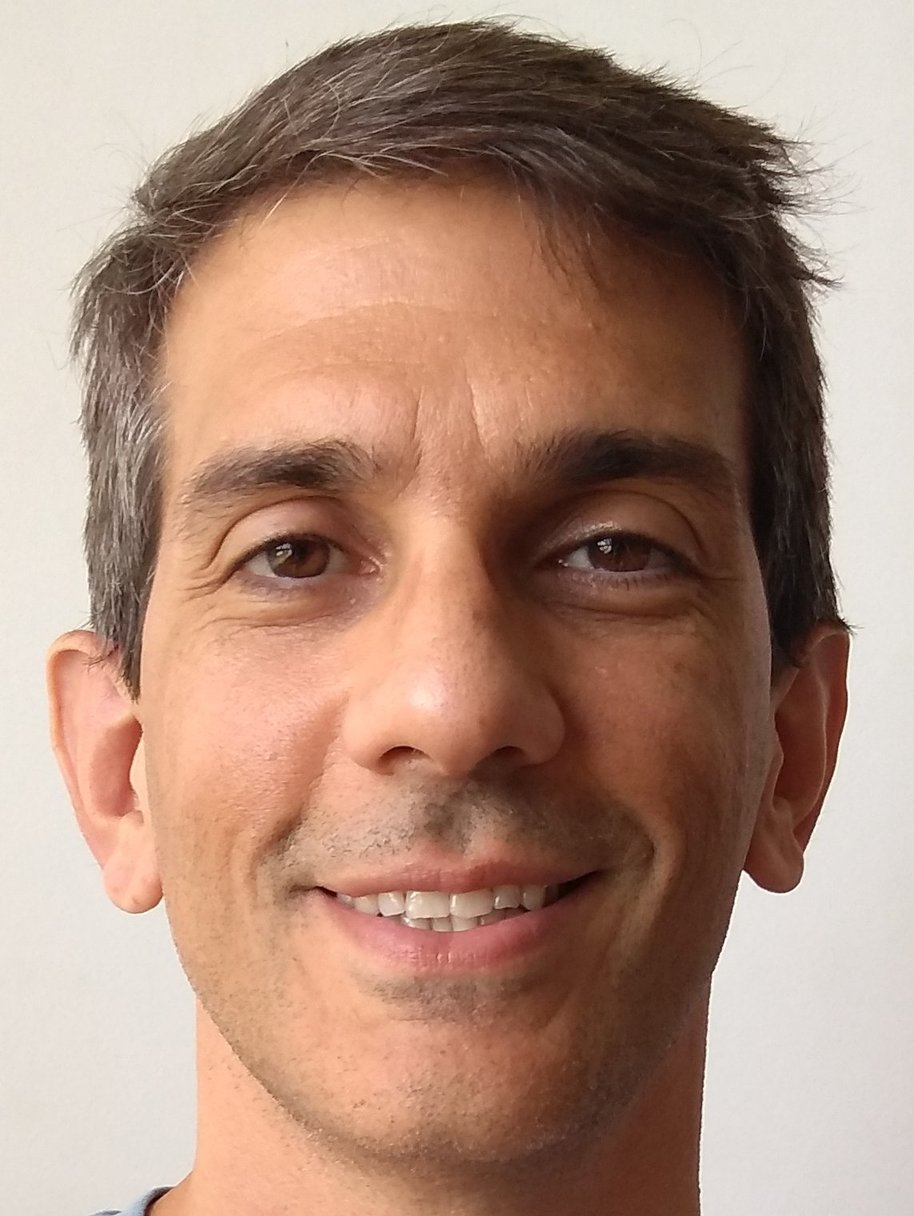
\includegraphics[width=0.13\textwidth]{images/marcelo.jpg}}
\date{ICSME 2021 (Virtual Event)\\{\scriptsize September 27 -- October 1}} % (optional, should be abbreviation of conference name)

%======================================================================================================

\begin{document}

\begingroup
\renewcommand{\disp}{}
\begin{frame}
	\titlepage
\end{frame}
\endgroup

\addtocounter{framenumber}{-1}

\begin{frame}{Context: software evolution and regression testing}
\vspace{-3.75mm}
\begin{center}
	{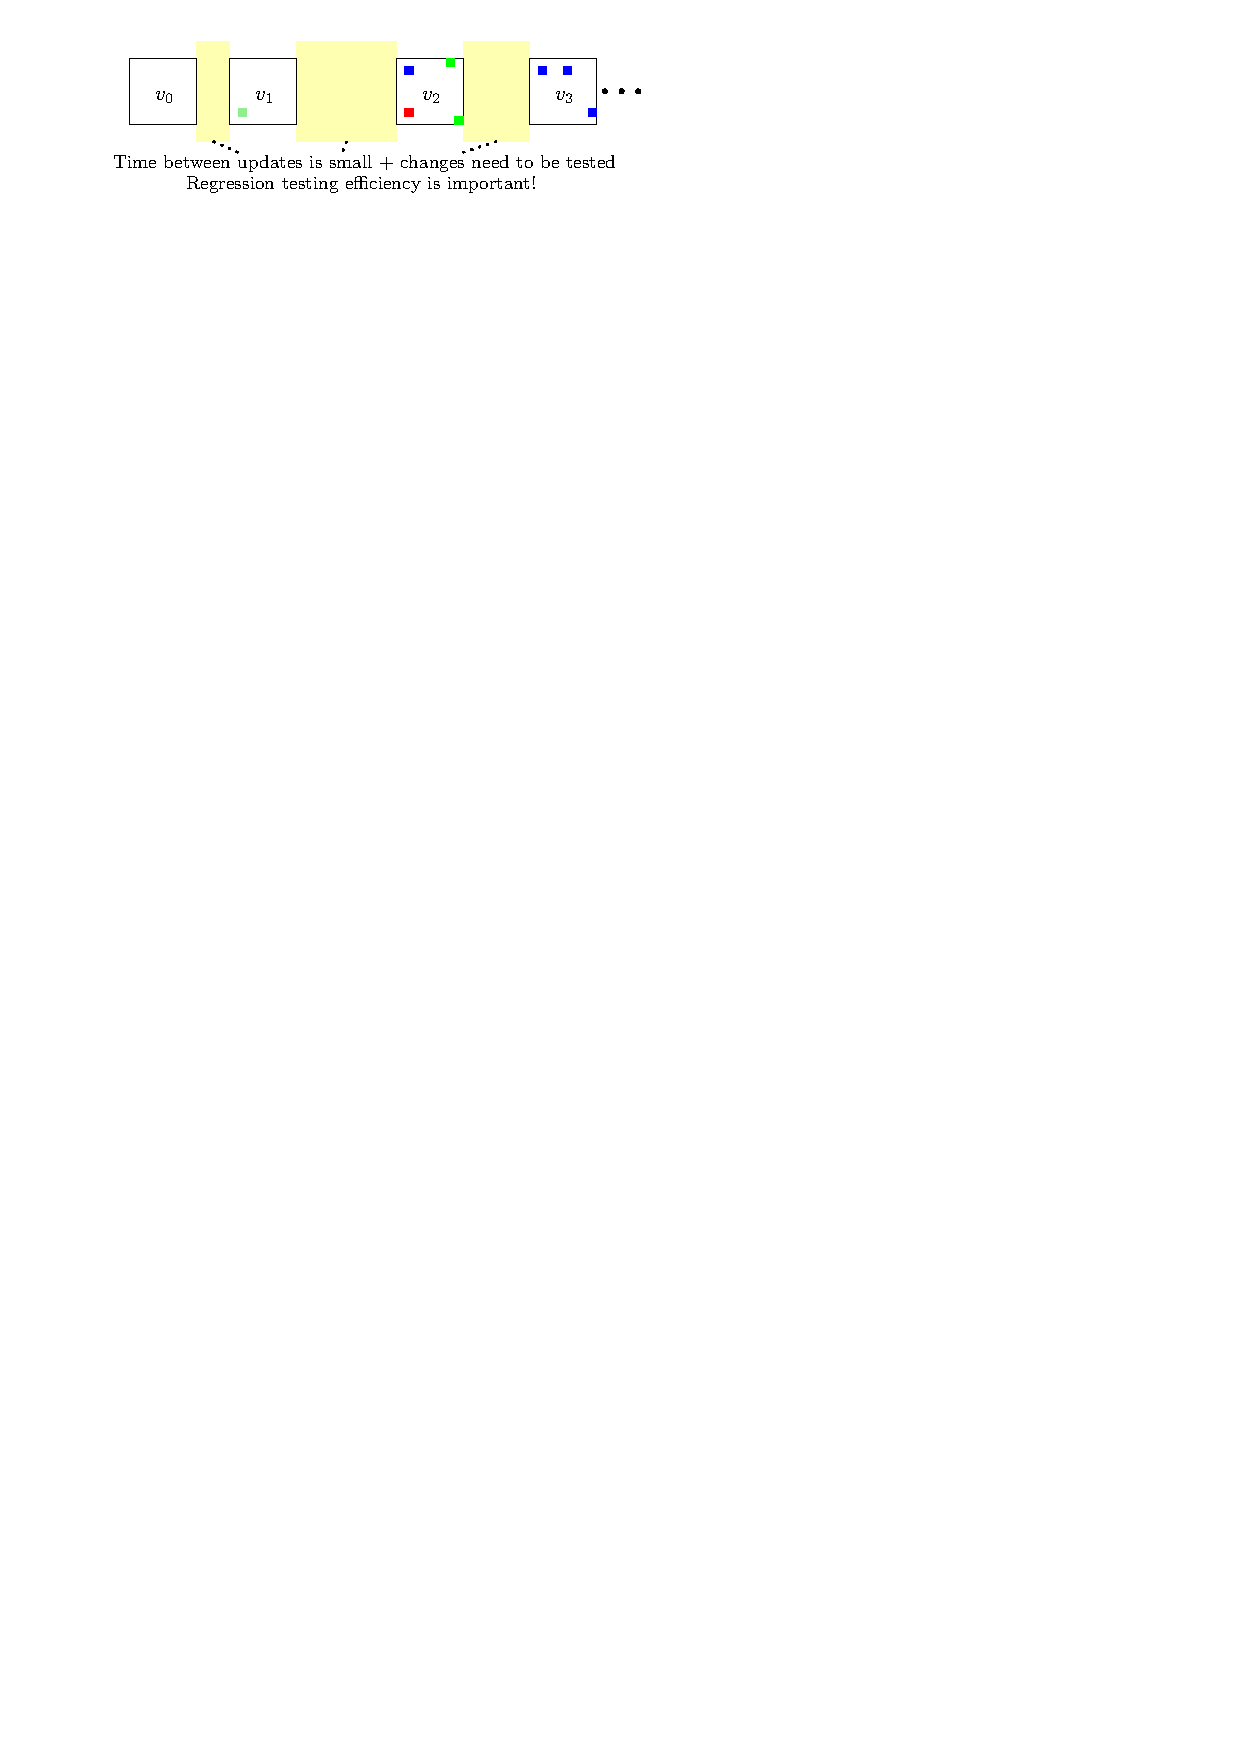
\includegraphics[width=\linewidth]{images/evolution.pdf}}
\end{center}
\vspace{-4mm}
\begin{center}
{\fontsize{10}{10}\selectfont
{\rsm \textbf{Regression testing}}: testing software changes for regression bugs.}
\end{center}\pause
\textit{Existing solutions}
\begin{itemize}
	\item[]{{\small Regression Test {\rsm Selection} (RTS)}\onslide<2->\footnotemark}\pause
	\item[]{{\small Regression Test {\rsm Prioritization} (RTP)}\onslide<3->\footnotemark}\pause
	\item[]{{\small Test Suite {\rsm Reduction} (TSR)}\onslide<4->\footnotemark}\pause
	\item[]{\textbf{\color{blue}\textit{Test execution parallelization}} (\textit{\color{red}is less explored}...).\onslide<5->\footnotemark}
\end{itemize}
\vfill
\only<2->{\footnotetext[1]{\fontsize{3.5}{3.5}\selectfont\textbf{Source}: M. Gligoric et al., \textit{Ekstazi: Lightweight Test Selection}, ICSE 2015.}}
\only<3->{\footnotetext[2]{\fontsize{3.5}{3.5}\selectfont\textbf{Source}: S. Elbaum et al., \textit{Test Case Prioritization: A Family of Empirical Studies}, TSE 2002.}}
\only<4->{\footnotetext[3]{\fontsize{3.5}{3.5}\selectfont\textbf{Source}: G. Rothermel et al., \textit{Empirical Studies of Test-Suite Reduction.}, STVR 2002.}}
\only<5->{\footnotetext[4]{\fontsize{3.5}{3.5}\selectfont\textbf{Source}: J. Candido et al., \textit{Test suite parallelization in open-source projects: A study on its usage and impact.}, ASE 2017.}}
\end{frame}

\begin{frame}{Two issues in test parallelization}
\begin{center}
{\color{blue}\textbf{Test dependencies} {\color{black}and} \textbf{data races}} give rise to {\color{red}\textbf{test flakiness}}.
\pause
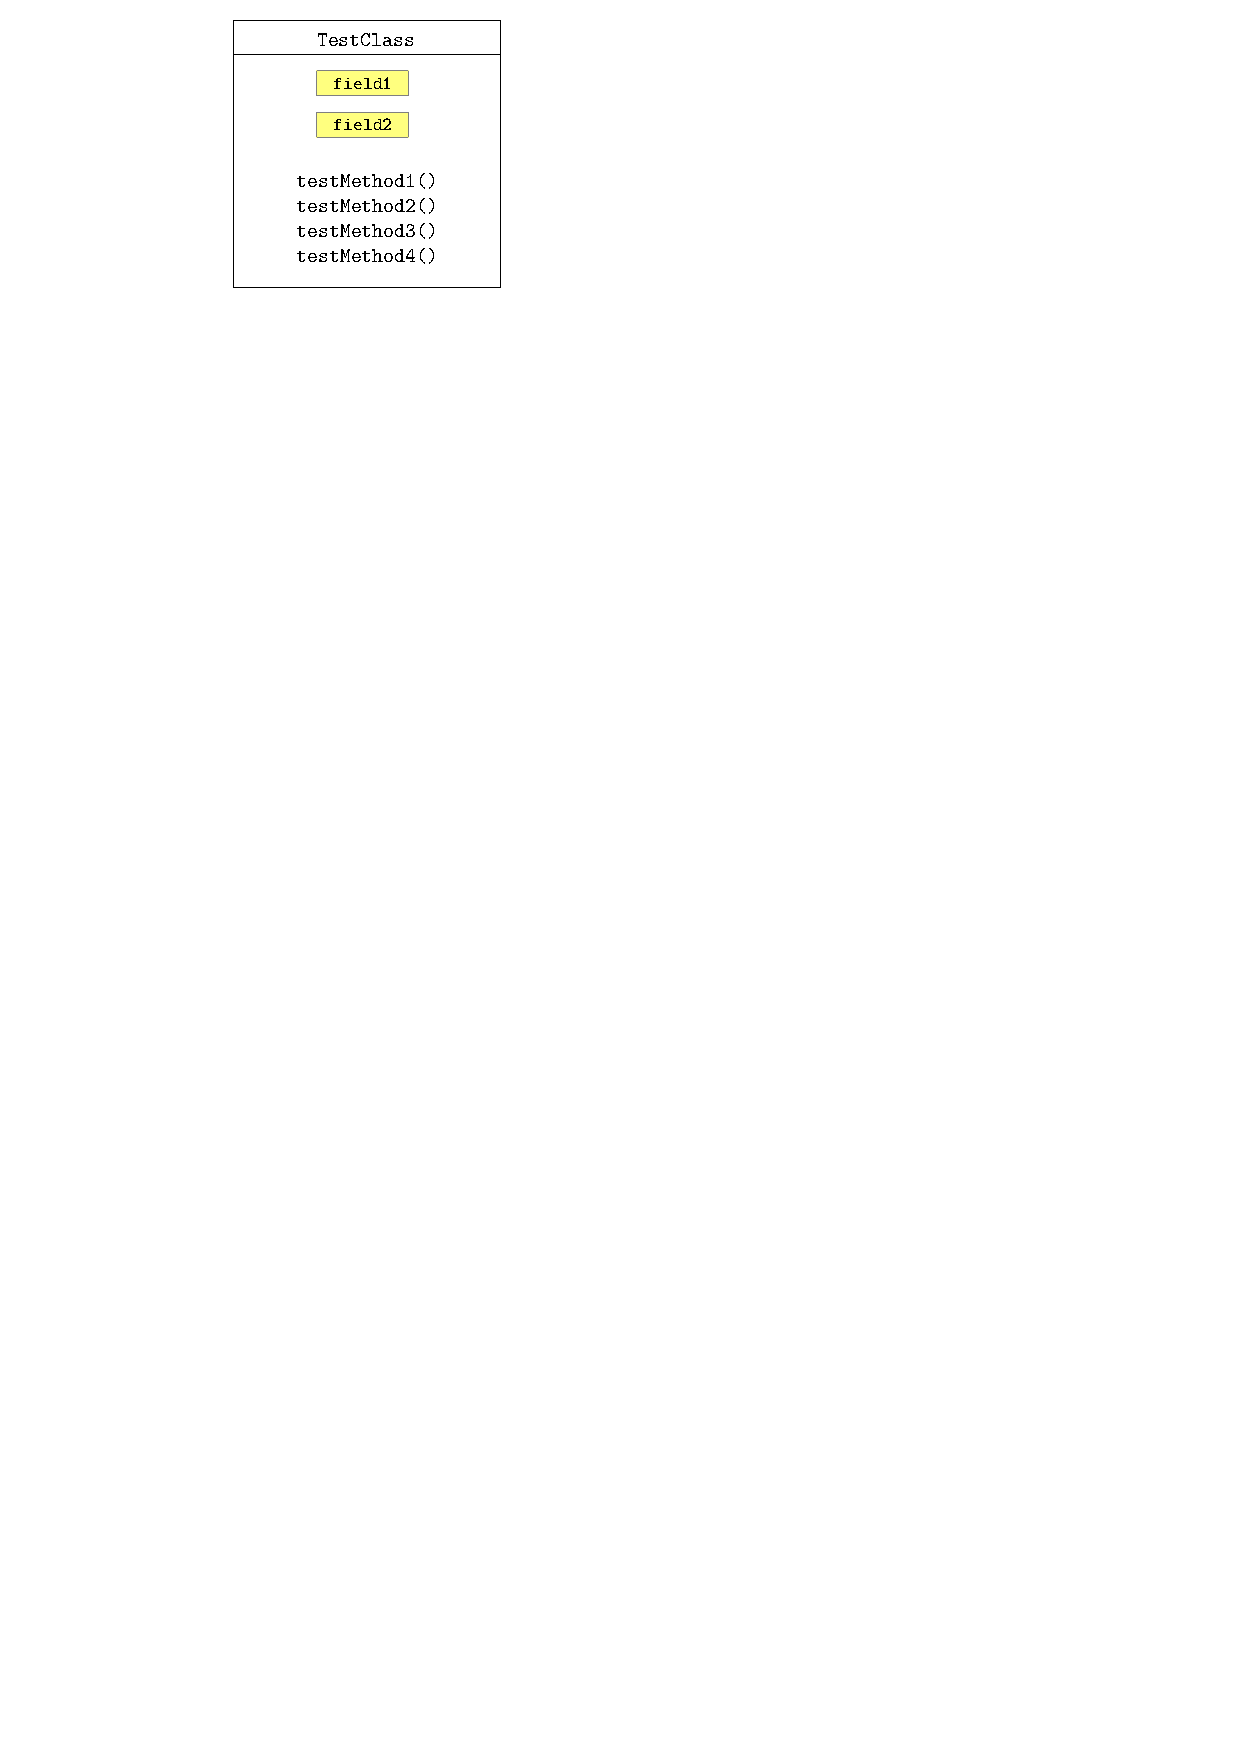
\includegraphics[width=0.6\linewidth,page=1]{images/flakes.pdf}
\end{center}
\end{frame}

\begin{frame}{Two issues in test parallelization}
	\begin{center}
{\color{blue}\textbf{\textit{Test dependencies}} {\color{black}and} \textbf{\color{black}data races}} give rise to {\color{red}\textbf{test flakiness}}.
		\includegraphics[width=0.6\linewidth,page=2]{images/flakes.pdf}
	\end{center}
\end{frame}

\begin{frame}{Two issues in test parallelization}
	\begin{center}
		{\textbf{Test dependencies} {\color{black}and} \textbf{\color{blue}\textit{data races}}} give rise to {\color{red}\textbf{test flakiness}}.
		\includegraphics[width=0.6\linewidth,page=3]{images/flakes.pdf}
	\end{center}
\end{frame}

\begin{frame}{Two issues in test parallelization}
	\begin{center}
{\color{blue}\textbf{Test dependencies} {\color{black}and} \textbf{data races}} give rise to {\color{red}\textbf{test flakiness}}.
		\includegraphics[width=0.8\linewidth,page=4]{images/flakes.pdf}
	\end{center}
{\color{white}
\centering
A topological sort would reveal a {\textbf{safe}} execution sequence.}
\end{frame}

\begin{frame}{Two issues in test parallelization}
	\begin{center}
		{\color{blue}\textbf{Test dependencies} {\color{black}and} \textbf{data races}} give rise to {\color{red}\textbf{test flakiness}}.
		\includegraphics[width=0.8\linewidth,page=7]{images/flakes.pdf}
	\end{center}
\centering
A {\rsm topological sort} would reveal a {\color{indiagreen}\textbf{safe}} execution sequence.\\\pause
But {\color{darkred}\textbf{prerequisite}} is \textit{test dependency detection}!
\end{frame}

\begin{frame}{Performance of a test dependency detector}
	\textit{State-of-the-art tool}: PRADET (ICST 2018)
	\vfill
	\fbox{\rsm \textbf{PRADET}}
	\begin{itemize}
		\fontsize{11}{11}\selectfont
		\item[]{{\textbf{Step 1} (costs $x$)}: {\rsm Sequential execution}}\pause
		\item[]{{\textbf{Step 2} (costs $y$)}: {\rsm Dynamic data-flow analysis}}\pause
		\item[]{{\textbf{Step 3} (costs $z$)}: {\rsm Dependency refinement}}\pause
	\end{itemize}
	\begin{center}
		\begin{tcolorbox}
			The overhead of {\rsm PRADET} was {\color{red} \textbf{substantially higher than sequential execution itself}} ($y+z>{x}$).\\\textit{\textbf{NOT practical} to use PRADET} to aid test parallelization!
		\end{tcolorbox}
	\end{center}
\end{frame}

\begin{frame}
	\begin{center}
		Our approach: \textbf{\tname}\\
		{\textbf{\rsm PA}rallel-\textbf{\rsm S}equential \textbf{\rsm T}est \textbf{\rsm E}xecution}\pause
		\vfill
		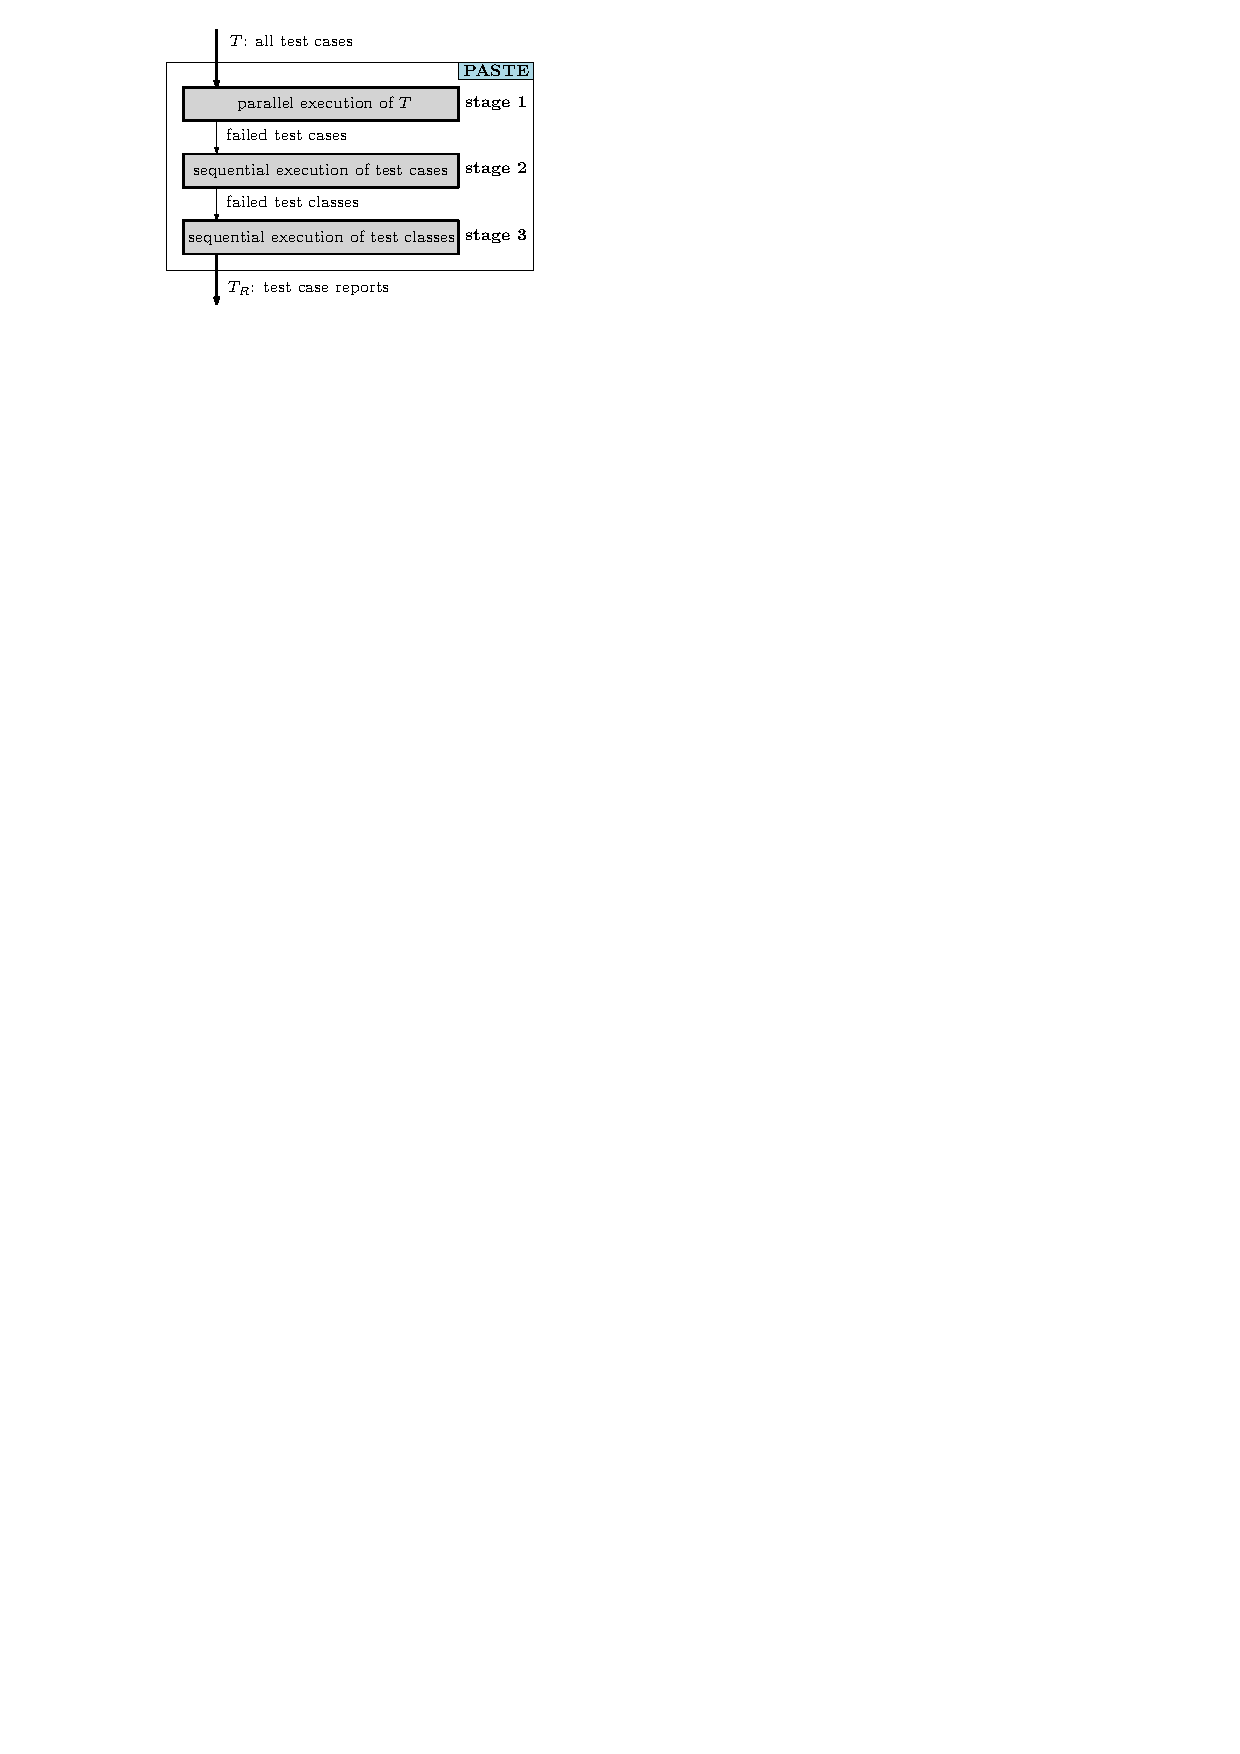
\includegraphics[width=0.8\linewidth,page=1]{images/soundy.pdf}
	\end{center}
\end{frame}

\begin{frame}{Stage 1: parallel execution}
	\centering 
	\includegraphics[width=0.65\linewidth,page=2]{images/soundy.pdf}
\end{frame}

\begin{frame}{Stage 1: parallel execution}
	\begin{center}
	{\includegraphics[width=0.5\linewidth,page=8]{images/flakes.pdf}}
	\end{center}
\centering
Execute the four test methods \textbf{\color{blue}in parallel}.\pause
\\Some test cases may fail!
\end{frame}

\begin{frame}{Stage 2: sequential re-execution of failed test cases}
	\centering 
	\includegraphics[width=0.65\linewidth,page=3]{images/soundy.pdf}
\end{frame}

\begin{frame}{Stage 2: sequential re-execution of failed test cases}
	\begin{center}
		\begin{minipage}{0.48\linewidth}
			\centering
			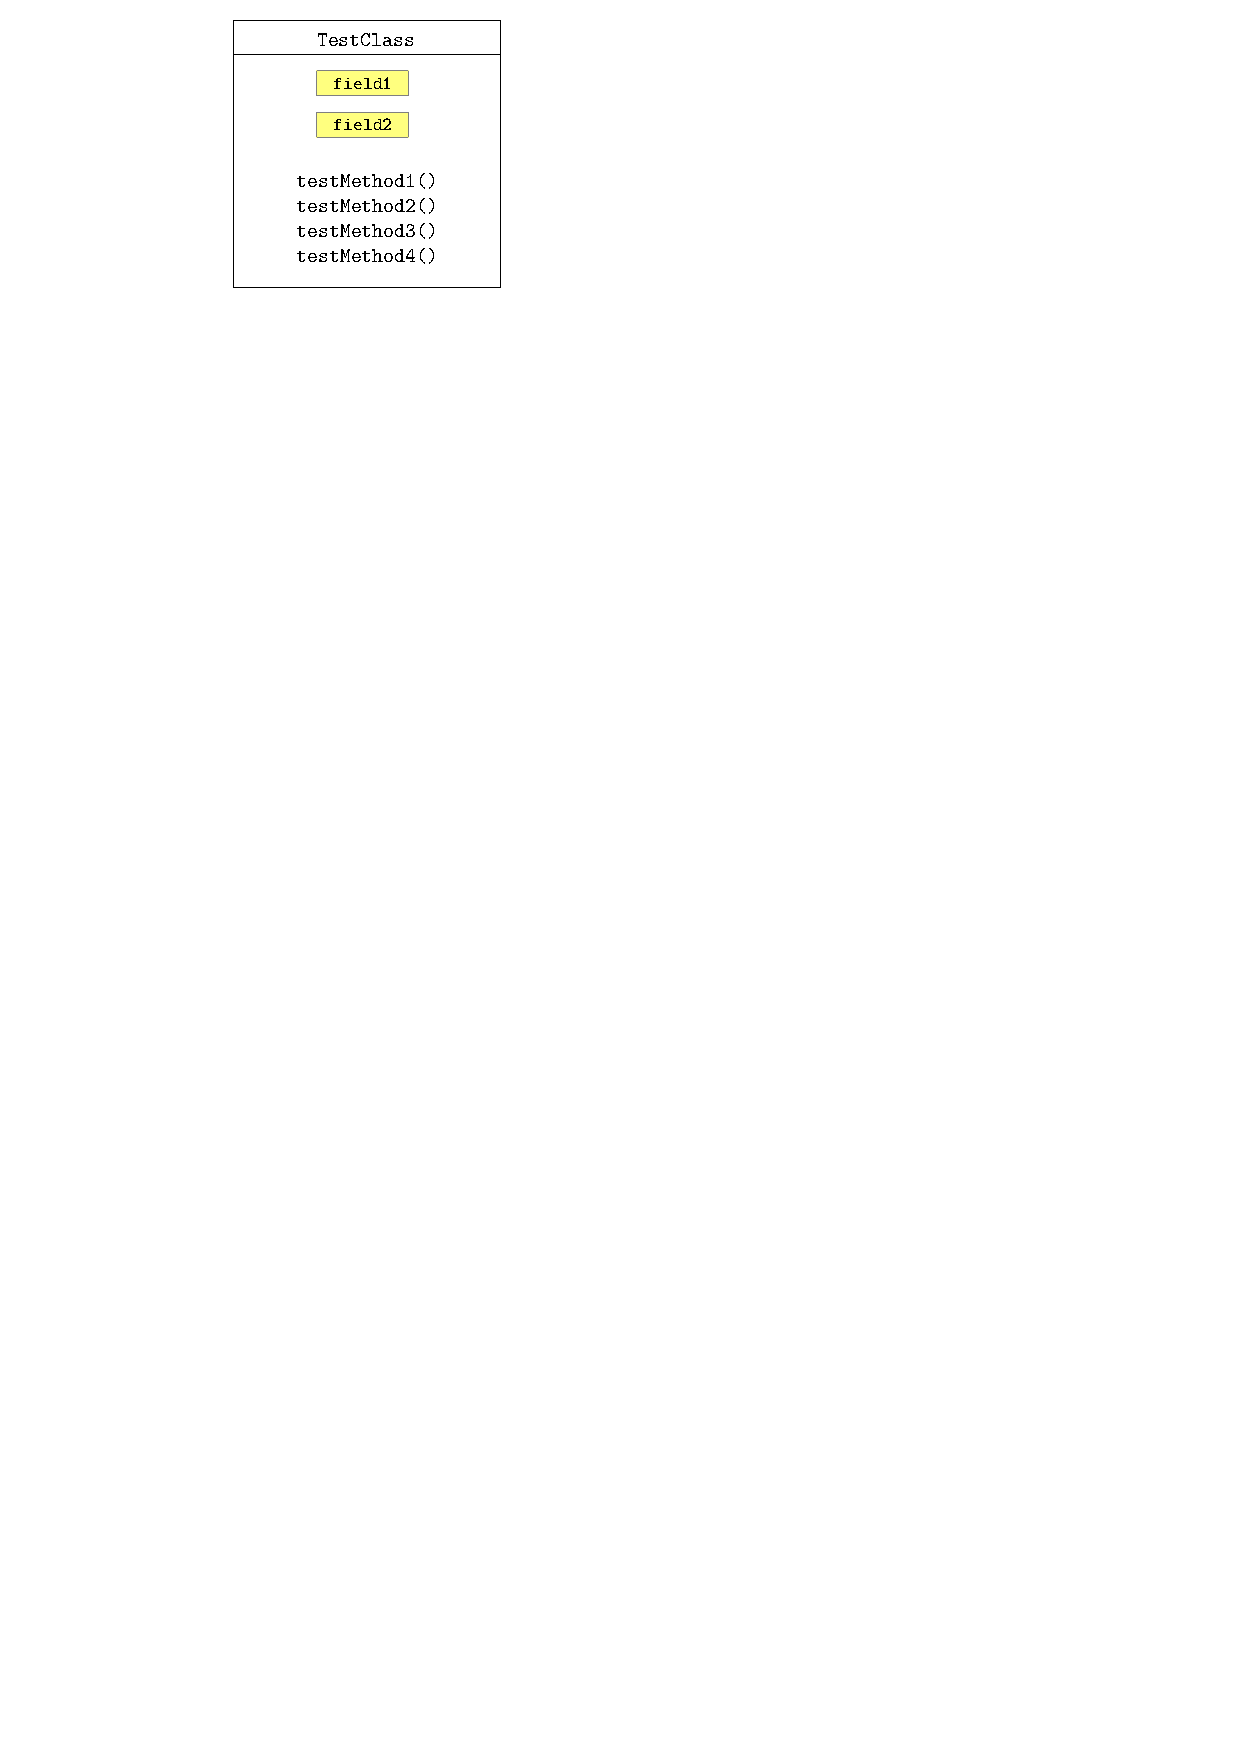
\includegraphics[width=0.85\linewidth,page=1]{images/flakes.pdf}
			%\vspace{1mm}
		\end{minipage}%
		\hfill
		\begin{minipage}{0.48\linewidth}
			\centering
			\includegraphics[width=0.85\linewidth,page=3]{images/flakes.pdf}
			%\vspace{1mm}
		\end{minipage}	
	\end{center}
	\textbf{Handle flakiness} through \textbf{sequential} {\color{blue}\textbf{re-execution}} of \textbf{\color{indiagreen}test cases} ({\textit{to circumvent {\color{red}\textbf{data races}}}}).\pause
	\vfill
	\begin{center}
	Some test cases may fail \textit{\textbf{again}}! \\
	Track their test class names.
	\end{center}
\end{frame}

\begin{frame}{Stage 3: sequential re-execution of failed test classes}
	\centering 
	\includegraphics[width=0.65\linewidth,page=4]{images/soundy.pdf}
\end{frame}

\begin{frame}{Stage 3: sequential re-execution of failed test classes}
\textbf{Handle flakiness} through \textbf{sequential} {\color{blue}\textbf{re-execution}} of \textbf{\color{indiagreen}test classes} ({\textit{to circumvent {\color{red}\textbf{broken test dependencies}}}}).
	\begin{center}
		\begin{minipage}{0.48\linewidth}
			\centering
			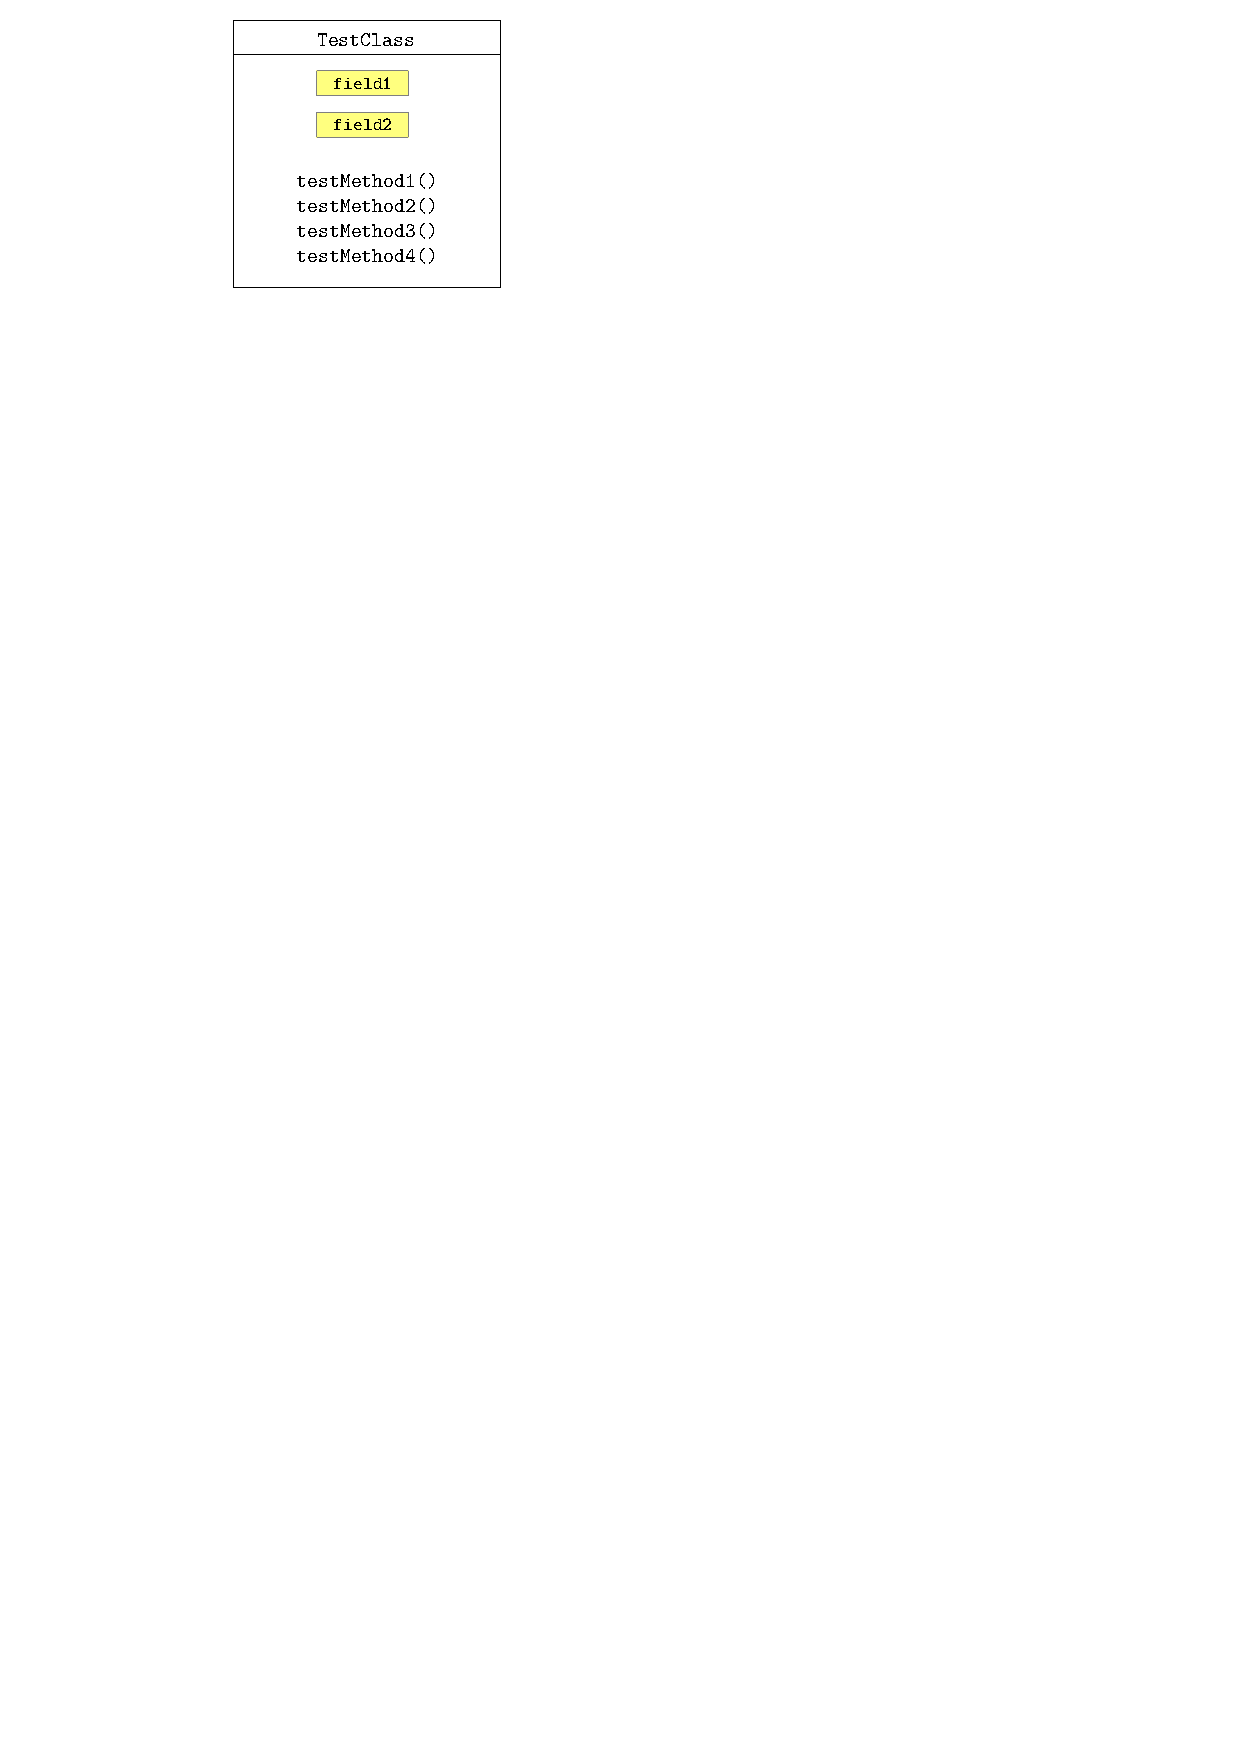
\includegraphics[width=0.85\linewidth,page=1]{images/flakes.pdf}
			%\vspace{1mm}
		\end{minipage}%
		\hfill
		\begin{minipage}{0.48\linewidth}
			\centering
			\includegraphics[width=0.85\linewidth,page=2]{images/flakes.pdf}
			%\vspace{1mm}
		\end{minipage}
	\end{center}
\pause
	\textbf{\tname} builds on the observation:\\
{\color{darkred} \textit{\textbf{broken test dependencies}}} that are manifested in parallel runs {\rsm \textit{\textbf{involve test cases from the same test class}}}.
\end{frame}

\begin{frame}{The spectrum of soundness in parallelization}
	
	{\textbf{\rsm Sound}: time invariant verdicts agree with sequential execution.}
	\begin{center}
		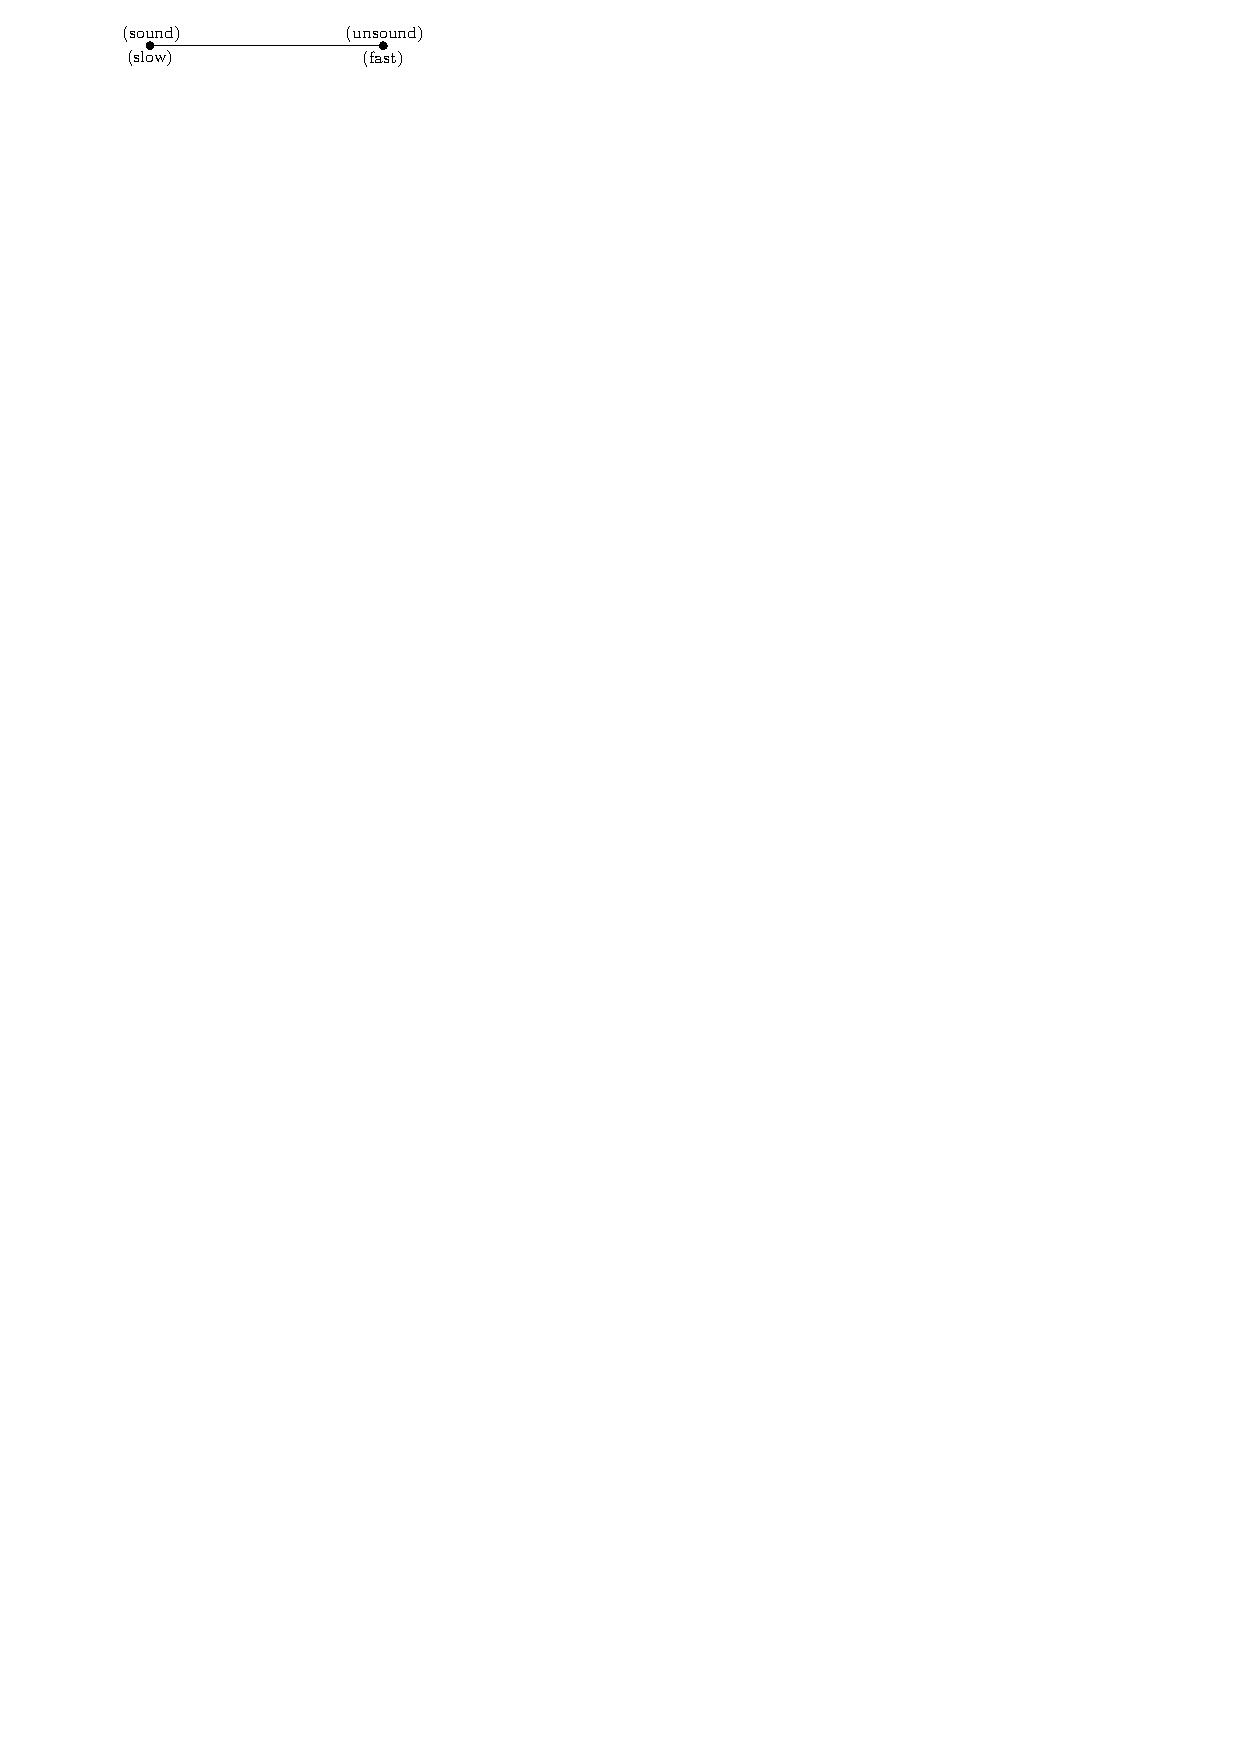
\includegraphics[width=0.8\linewidth,page=1]{images/spectrum.pdf}
		\vfill
		{\color{white}\tname{} does not provide the soundness guarantee but is reasonable enough to yield end-to-end acceleration!}
	\end{center}
\end{frame}

\begin{frame}{The spectrum of soundness in parallelization}
	
	{\textbf{\rsm Sound}: time invariant verdicts agree with sequential execution.}
	\begin{center}
		\includegraphics[width=0.8\linewidth,page=2]{images/spectrum.pdf}
		\vfill
		{\color{blue}\tname{} does not provide the soundness guarantee but is reasonable enough to yield end-to-end acceleration!}
	\end{center}
\end{frame}

\begingroup
\renewcommand{\disp}{}
\begin{frame}
	\begin{center}
		Experimental Setup
	\end{center}
\end{frame}
\endgroup
\addtocounter{framenumber}{-1}

\begin{frame}{Experimental Setup}
	\begin{itemize}
		\item[]{\textbf{\underline{Hardware}}: \textbf{\rsm \NumCPUs\ CPUs} (\textbf{\rsm \NumCores\ cores}, with \textbf{\rsm 2 threads per core}).}\pause
		\item[]{\textbf{\underline{Software}}: GNU \textbf{\rsm {Bash}} \BashVersion, and \textbf{\rsm {Maven}} \MavenVersion.}\pause
		\item[]{\textbf{\underline{Subjects}}: \textbf{\rsm \NumProjects\ Java projects} that use \textbf{\rsm {Maven}} and have at least \NumStars\ stars and \NumTests\ tests.}\pause
		\item[]{\textbf{\underline{No failures}}: Reran each test suite \NumRepeatsManifest\ times to \textbf{\rsm identify} and \textbf{\rsm eliminate tests failing} due to \textbf{\rsm non-determinism}.}
	\end{itemize}
\end{frame}

\begingroup
\renewcommand{\disp}{}
\begin{frame}
	\begin{center}
		Research Questions
	\end{center}
\end{frame}
\endgroup
\addtocounter{framenumber}{-1}

\begin{frame}{RQ1 (feasibility \#1)}
	\textbf{\textit{Is it {\rsm feasible to use parallelization} options provided by the build system ``{\rsm out of the box}'' to run test suites?}}\pause
	\begin{center}
		\begin{tcolorbox}
			In \NumProjectsParExecFailsPercentage\% of the projects, no parallel configurations enabled a clean execution. Searching for the {\color{red}\textbf{parallel configuration for a clean execution is INFEASIBLE in general}}.
		\end{tcolorbox}
	\end{center}
\end{frame}

\begin{frame}{RQ2 (feasibility \#2)}
	\textbf{\textit{Is it {\rsm practical to use a test dependency analyzer} to partition test sets as to enable {\rsm sound} parallel execution?}}\pause
	\begin{center}
		\begin{tcolorbox}
			The runtime overhead of PRADET was substantially higher than that of the sequential execution itself. \textbf{\color{red} NOT PRACTICAL to use PRADET to aid test parallelization}.
		\end{tcolorbox}
	\end{center}
\end{frame}

\begin{frame}{RQ3 (effectiveness \#1)}
	\textbf{\textit{How {\rsm reliable} is \tname?}}
	\begin{center}\pause
		\begin{tcolorbox}
			Effective to circumvent the test flakiness provoked by test parallelization. There were \textbf{\color{red}no cases of provoked failure that ``survived'' the third stage} of \tname.
		\end{tcolorbox}
	\end{center}
\end{frame}

\begin{frame}{RQ4 (effectiveness \#2)}
	\textbf{\textit{What are the {\rsm speedups obtained} with \tname?}}
	\begin{center}\pause
		\begin{tcolorbox}
			We observed speedups in \FrequencySpeedups\% of the projects. The {\color{red}\textbf{configuration} \texttt{\textbf{classes}}} performed the best: {\color{red} \textbf{median}~\textbf{\SpeedupClassesMedian{}x}} (best: \SpeedupClassesMax{}x, average: \SpeedupClassesAvg{}x, worst: \SpeedupClassesMin{}x).
		\end{tcolorbox}
	\end{center}
\end{frame}

\begingroup
\renewcommand{\disp}{}
\begin{frame}
	\begin{center}
		Related Work
	\end{center}
\end{frame}
\endgroup
\addtocounter{framenumber}{-1}

\begin{frame}{Most relevant related work}
	\begin{center}
		\fontsize{7.5}{7.5}
		{	
			\selectfont
			\setlength{\tabcolsep}{0.9mm}
			\centering
			\begin{tabular}{l|l|l}
				\hline
				{\textbf{Work--venue}} & {\textbf{Description}} & {\textbf{Relation}}\\
				\hline
				{} & {} & {} \\
				{{\rsm ElectricTest}--FSE 2015} & {Tracks {\rsm test dependencies} on global} & {Complementary}\\
				{} & {resources + {\rsm distributed parallelization}.} & {} \\
				{} & {} & {} \\
				\hline\pause
				{} & {} & {} \\
				{{\rsm ParTeCL}--ISSTA 2017} & {Transforms code to GPU kernels} & {Domain specific}\\
				{} & {for {\rsm GPU level parallelization}.} & {Yet to explore} \\
				{} & {} & {} \\
				\hline\pause
				{} & {} & {} \\
				{{\rsm TEDD}--FSE 2019} & {NLP-based {\rsm web test dependency} detector} & {Domain specific}\\
				{} & {tracks client-server {\rsm network operations}.} & {Yet to explore} \\
				{} & {} & {} \\
				\hline
			\end{tabular}
		}	
	\end{center}
	\centering
	%{\fontsize{9}{9}\selectfont We \underline{\textit{may get}} a {\color{indiagreen}\textbf{good speedup}}.}
\end{frame}

\begin{frame}{Conclusions}
	\begin{itemize}
		\item[]{\footnotesize We discussed {\rsm \textbf{\tname{}}}, a lightweight approach to {\rsm \underline{parallelize execution}} of test suites through the {\rsm \underline{sequential re-execution} of \textit{test cases}} (\textit{to avoid data races}) and the {\rsm \underline{sequential re-execution} of \textit{test classes}} (\textit{to avoid broken test dependencies}).}
	\end{itemize}
	\begin{center}
		\begin{figure}[!htb]
			\centering
			\begin{minipage}{0.475\textwidth}
				\centering
				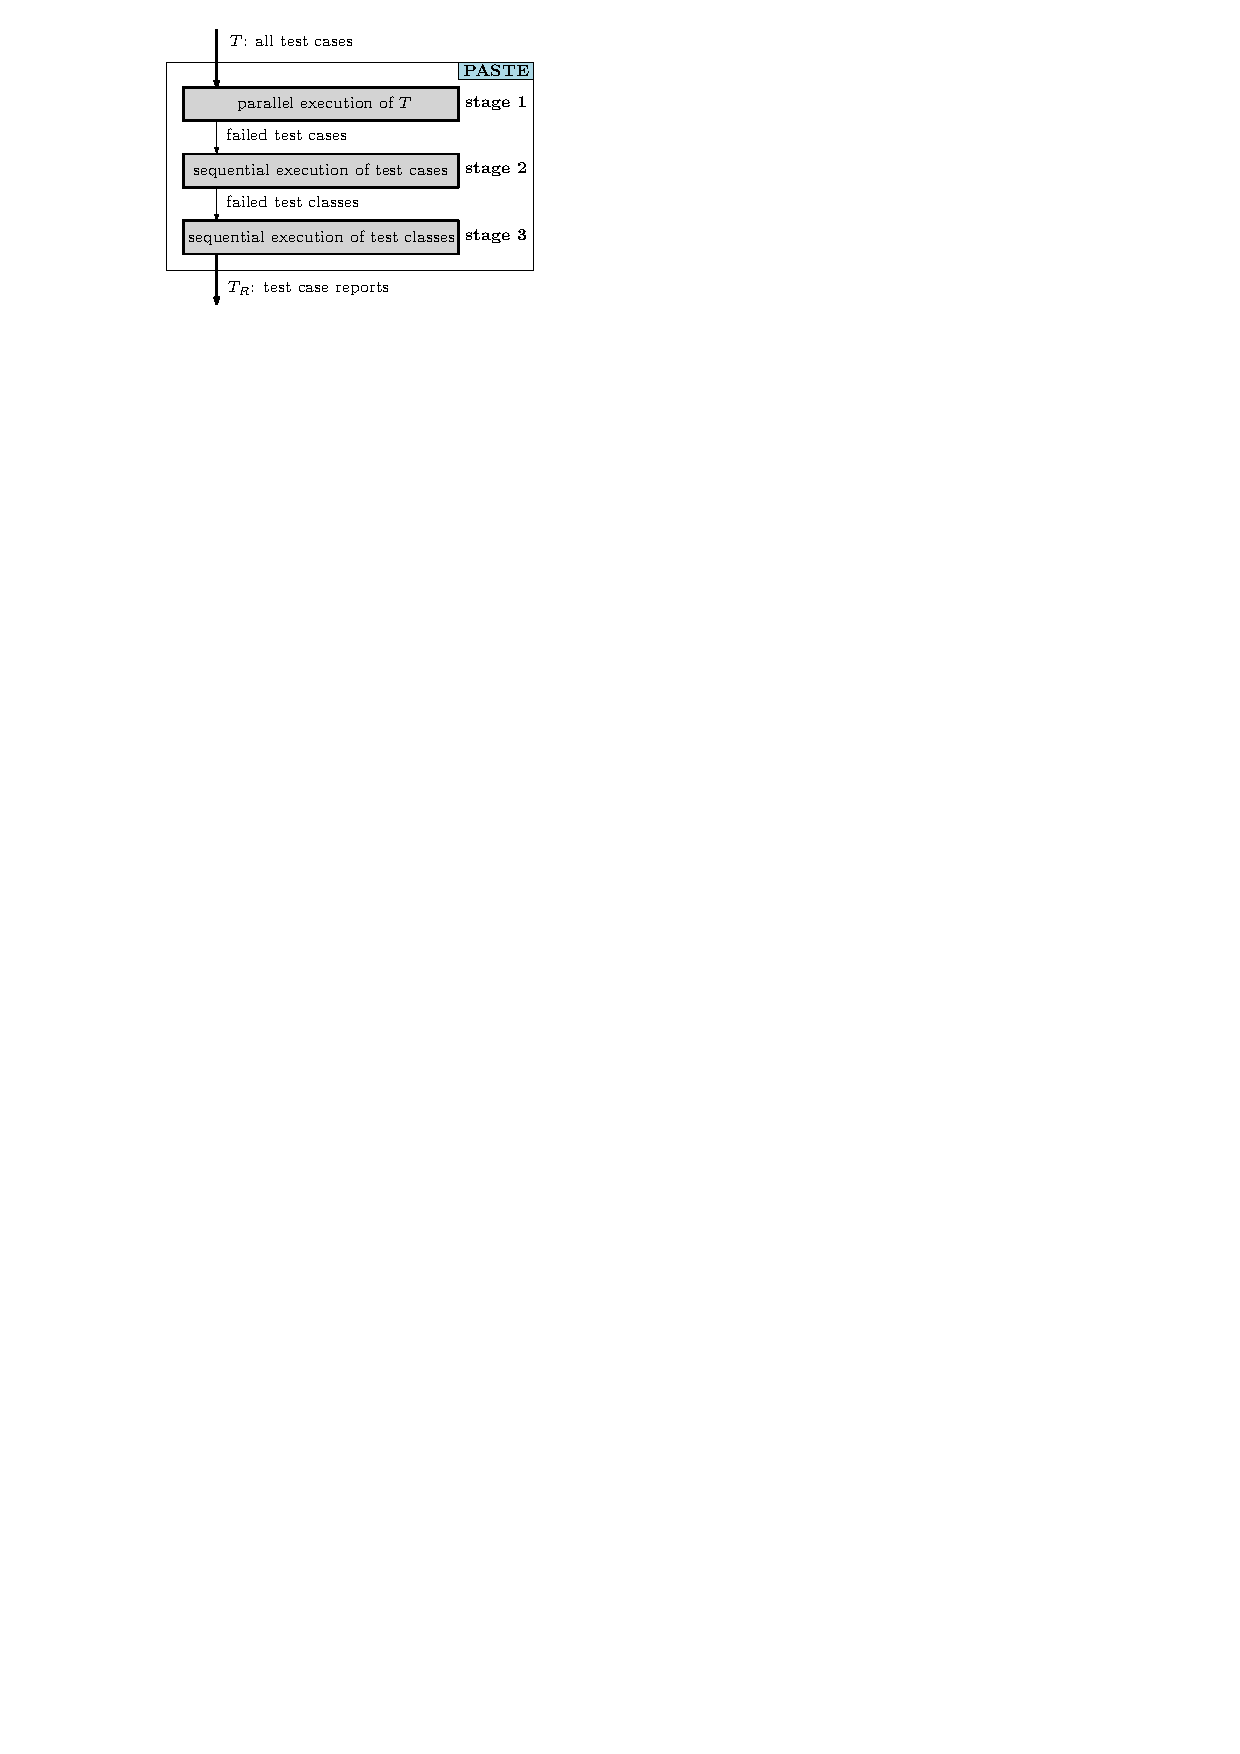
\includegraphics[width=\linewidth]{images/soundy.pdf}	
			\end{minipage}%
			\pause
			\begin{minipage}{0.5\textwidth}
				\centering
				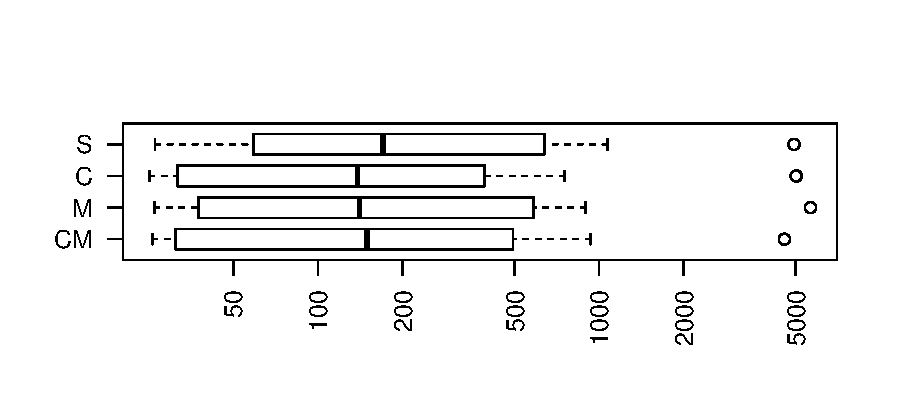
\includegraphics[width=1.175\linewidth]{images/time.pdf}\vspace{-1cm}
				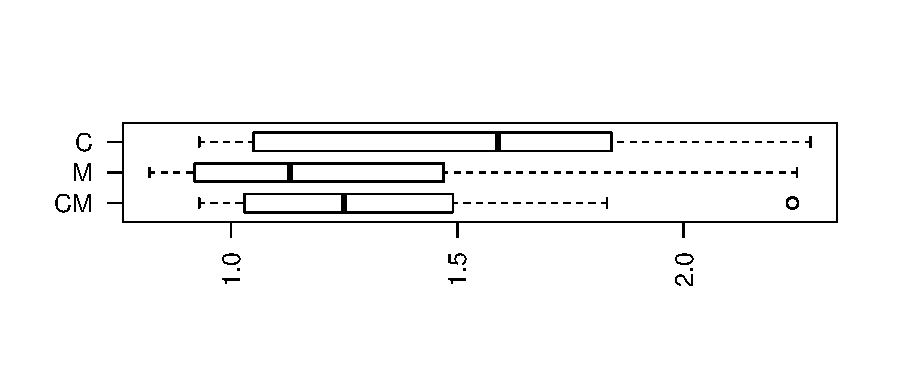
\includegraphics[width=1.175\linewidth]{images/speedup.pdf}	
			\end{minipage}
		\end{figure}
		\includegraphics[width=0.5\linewidth,page=2]{images/spectrum.pdf}
		\pause
		\hfill
		\begin{Large}
			Thank You
		\end{Large}
		\vfill
		\begin{footnotesize}
			Artifacts: \url{https://github.com/STAR-RG/paste}
		\end{footnotesize}
	\end{center}
\end{frame}

%======================================================================================================

\REM{
	
\renewcommand{\disp}{}

\appendix
\backupbegin

\begin{frame}
	\begin{center}
		{\huge Backup Slides}
	\end{center}
\end{frame}

\begin{frame}{Test parallelization levels}
	\centering
	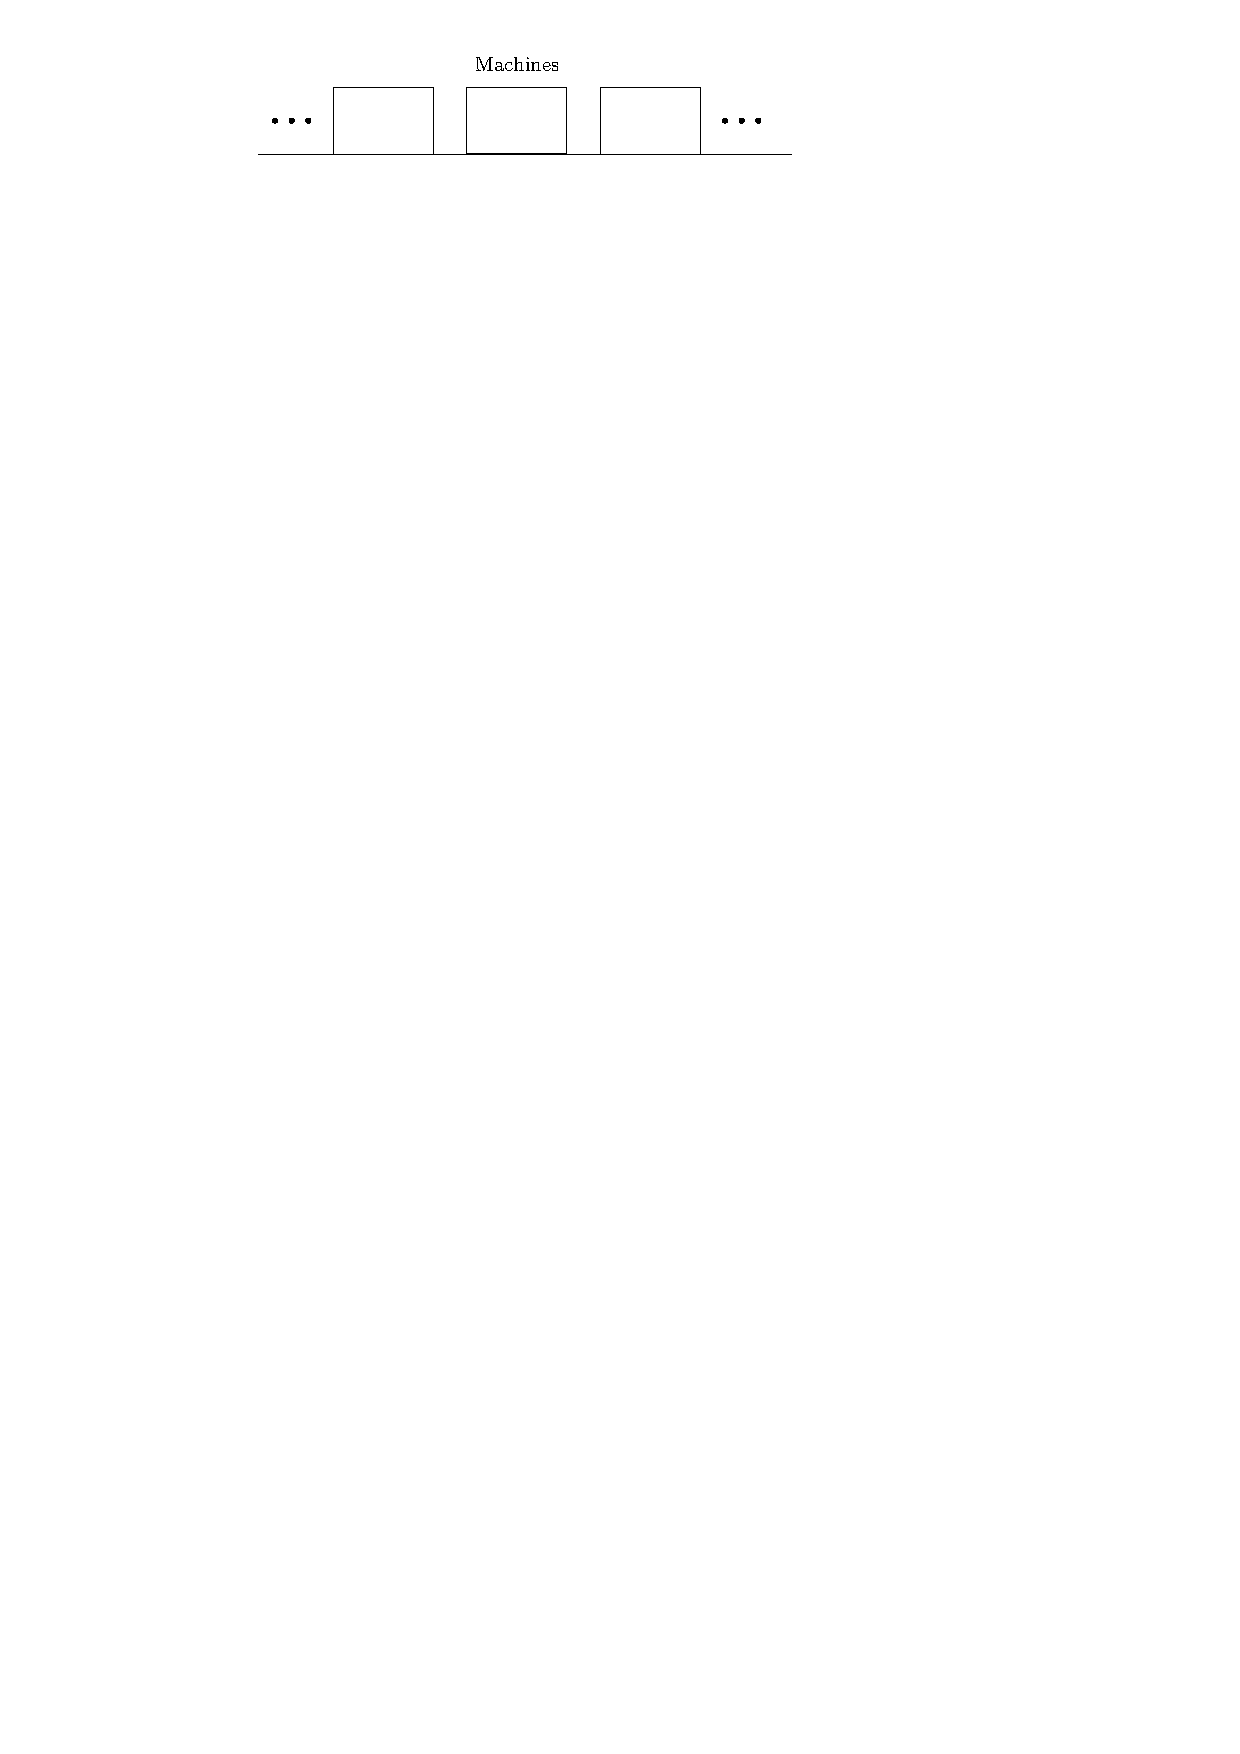
\includegraphics[width=\linewidth,page=1]{images/intro.pdf}
	\vfill
	{\color{white}In this work, we focus on \textit{CPU} and \textit{thread} level parallelism.}
	\vfill
	\vfill
	{\fontsize{5}{5}\selectfont\textbf{Source}: J. Candido et al., \textit{Test suite parallelization in open-source projects: A study on its usage and impact}, ASE 2017.}
\end{frame}

\begin{frame}{Test parallelization levels}
	\centering
	\includegraphics[width=\linewidth,page=2]{images/intro.pdf}
	\vfill
	{\color{white}In this work, we focus on \textit{CPU} and \textit{thread} level parallelism.}
	\vfill
	\vfill
	{\fontsize{5}{5}\selectfont\textbf{Source}: J. Candido et al., \textit{Test suite parallelization in open-source projects: A study on its usage and impact}, ASE 2017.}
\end{frame}

\begin{frame}{Test parallelization levels}
	\centering
	\includegraphics[width=\linewidth,page=3]{images/intro.pdf}
	\vfill
	{\color{black}In this work, we focus on \textit{CPU} and \textit{thread} level parallelism.}
	\vfill
	\vfill
	{\fontsize{5}{5}\selectfont\textbf{Source}: J. Candido et al., \textit{Test suite parallelization in open-source projects: A study on its usage and impact}, ASE 2017.}
\end{frame}

\begin{frame}{The rationale behind \textbf{\tname}}
	
	\textbf{\tname} builds on the observation:\\
	{\rsm \textit{\textbf{broken test dependencies}}} that are manifested in parallel runs {\rsm \textit{\textbf{involve test cases from the same test class}}}.
	\begin{center}
		\begin{minipage}{0.48\linewidth}
			\centering
			\includegraphics[width=\linewidth,page=5]{images/flakes.pdf}
			%\vspace{1mm}
		\end{minipage}%
		\hfill
		\begin{minipage}{0.48\linewidth}
			\centering
			\includegraphics[width=\linewidth,page=6]{images/flakes.pdf}
			%\vspace{1mm}
		\end{minipage}\pause
		\begin{tcolorbox}
			\vfill
			\textbf{Handle flakiness} in test suites through:
			\begin{itemize}
				\item{\textbf{sequential} {\color{blue}\textbf{re-execution}} of \textbf{\color{indiagreen}test cases} \\({\textit{to avoid {\color{red}\textbf{data races}}}}).}
				\item{\textbf{sequential} {\color{blue}\textbf{re-execution}} of \textbf{\color{indiagreen}test classes} \\({\textit{to avoid {\color{red}\textbf{broken test dependencies}}}}).}
			\end{itemize}
		\end{tcolorbox}
	\end{center}
\end{frame}

\begin{frame}{RQ4 (effectiveness \#2)}
	\vspace{-1.2cm}
	\begin{figure}
		\centering
		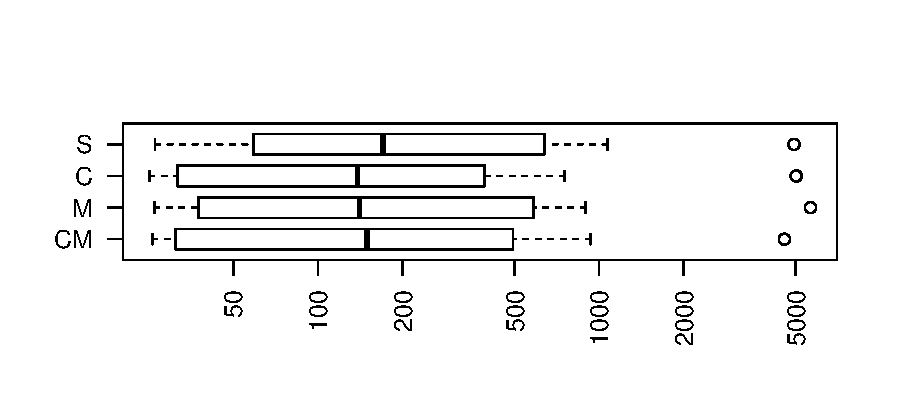
\includegraphics[width=\linewidth]{images/time.pdf}
		\vspace{-1.4cm}
		\caption*{Distribution of {\rsm \textbf{\tname{} running times (seconds)}} for Sequential (S) and each configuration (Classes (C), Methods (M), ClassesMethods (CM)).}
	\end{figure}
	\vspace{-1.25cm}\pause
	\begin{figure}
		\centering
		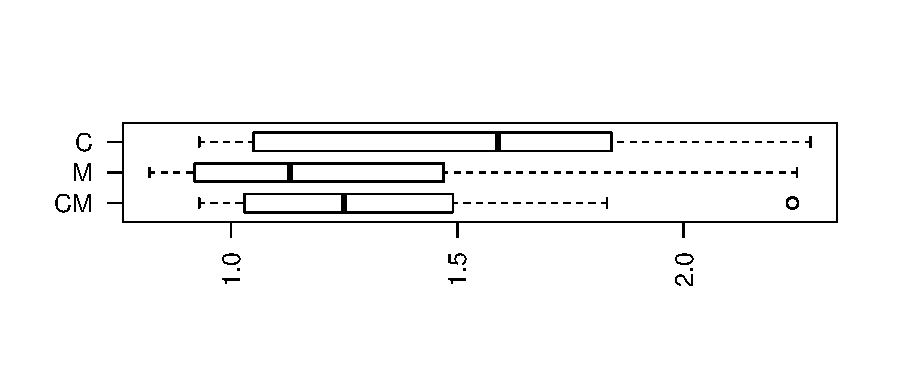
\includegraphics[width=\linewidth]{images/speedup.pdf}
		\vspace{-1.6cm}
		\caption*{Distribution of {\rsm \textbf{speedups}} for each configuration (Classes (C), Methods (M), ClassesMethods (CM)).}
	\end{figure}
\end{frame}

\backupend

}

\end{document}